\chapter{Saber: delegating transport layer security to browsers}

\section{Introduction}
\label{sec:intro-saber}

Transport Layer Security (TLS) is a cryptographic protocol designed to provide
end-to-end communication security between two parties, even in the presence of
active man-in-the-middle adversaries. It has since become the standard for
providing secure communication on the Internet and is used for several
sensitive applications such as banking, email, instant messaging, shopping,
etc. Usage of TLS is most commonly seen in securing web traffic in the form of
HTTPS. When implemented correctly, HTTPS guarantees confidentiality, integrity,
and authenticity of all web communication between two parties. Further, there
are additional mechanisms such as \emph{strict transport security} (HSTS),
\emph{public key pinning} (HPKP), \emph{online certificate status protocol}
(OCSP) stapling, and \emph{certificate transparency} (CT), that improve the
security of HTTPS. However implementing HTTPS and all the supporting security
mechanisms correctly has proven to be a challenge for most applications.

While browsers are not free from TLS bugs, they have been patched over time
through extensive amounts of penetration testing. They have further been the
pioneers of modern HTTPS standards and are the first to implement them into
practice. Previous work has found that non-browser applications in particular
have struggled with validating TLS certificates\cite{dangerous}. We also
further find that they lag behind in other web security practices such as HSTS,
HPKP, and certificate revocation checking. Despite this, usage of non-browser
software such as package managers, wget/curl, and language specific request
libraries, is prominent. These applications and libraries support TLS and hence
provide the impression of giving security to the user, but they fail to live up
to that promise. We find that browsers such as Chrome and Firefox implement not
only secure validation of TLS certificates in general, implement mechanisms
such as HSTS, HPKP, and verification of revoked certificates, but also have
dynamic protection against identified malware and dangerous binaries. They are
also better at displaying security warnings to the user in a transparent
manner.

The issues with improper implementation of TLS for non-browser applications are
due to both the complexity of the protocol, lack of general understanding of
TLS, and not having the same security expertise and engineering resources for
development as browsers do. Solving these issues would be a monumental task and
would require widespread education of the importance of properly implementing
communication security, along with the expense of recruiting security experts
for every application that requires using TLS, which may not be feasible for
several applications that are maintained by individual developers but are
nonetheless popular.

We propose a new way to build non-browser applications that allows developers
to use the TLS protocol for web security but does not require the expertise
needed to implement TLS verification correctly. Our method involves delegating
the handling of connection security to browsers, so the non-browser application
deals only with application layer logic. This allows non-browser applications
to get connection security for free from browsers. This also lets them take
advantage of any mechanisms that browsers implement to harden TLS security
(such as HSTS, HPKP, etc.) for free as well. We have built a prototype version
of wget using this method as a proof of concept. Our application is able to
validate proper TLS connections without writing any code that requires a deep
knowledge of the TLS protocol.

This chapter is organized as follows: In \Cref{sec:background-saber}, we
discuss the background material related to TLS and HTTPS, the various existing
problems with the ecosystem and how browsers have taken steps to solve them. In
\Cref{sec:problems-saber} we look at some non-browser applications, in
particular \emph{wget} to see how they compare to modern browsers in terms of
connection security. In \Cref{sec:solution-saber}, we present the design of a
library that delegates connection security to the browser. In
\Cref{sec:swget-saber}, we present \emph{swget} as a prototype implementation
of wget that provides better connection security by delegating TLS to browsers.
In \Cref{sec:conclusion-saber}, we conclude. In \Cref{sec:related-saber}, we
discuss related work.
% TODO: write sections descriptions better


\section{Background}
\label{sec:background-saber}

In this section, we present a brief description TLS, HTTPS, and additional security
mechanisms that harden the HTTPS ecosystem.

\subsection{TLS}
Transport Layer Security (TLS) is a cryptographic protocol that has been
established as the standard method of secure, encrypted communication over the
Internet. TLS aims to provide \emph{Authenticated Encryption} which requires the
following key properties-
\begin{itemize}
  \item \textbf{Confidentiality:} All communication between two parties is
  encrypted such that no information about the contents of the communication is
  leaked to an adversary.

  \item \textbf{Integrity:} An adversary must not be able to change the
  contents of the communication between the two parties in any way.

  \item \textbf{Authenticity:} The two communicating parties can verify the
  identity of each other (or atleast one party) through some certificate, and
  ensure that the messages exchanged are from each other. As such, an adversary
  cannot pretend to be one of the comunicating parties.
\end{itemize}

TLS provides these security guaranties underneath the application layer,
Several application layer protocols such as HTTPS, IMAPS, XMPP, and SMTP use TLS
to provide end-to-end security.

\subsection{HTTPS}
HTTPS (or "HTTP over TLS") is a protocol which secures HTTP traffic within a
connection encrypted by the TLS protocol. It is mainly used for authenticating
a website and securing communication between the website and its users.

\subsection{Strict Transport Security}
While HTTPS protects users from active man-in-the-middle attackers, the
protection only applies if the client actually makes an HTTPS web request.
There are certain clients or browser extension that force every request to be
HTTPS, but with a large portion of the web only accessible over HTTP, such a
client is infeasible and would block access to a significant portion of the
Internet for users.

Secure connection to a domain that does serve over HTTPS can only be guaranteed
if the initial web request made by the client was over HTTPS. Even if the
domain redirects from HTTP to HTTPS for partial or all of the web requests
that it serves, an active man-in-the-middle attacker could intercept that
redirect and replace it with a forged accept response pretending to be the
server. As a result, the attacker could make it so that the client never
actually switches to an HTTPS connection and remains vulnerable. This class of
attacks is commonly known as \emph{SSL Stripping}.

To combat this problem, servers now serve \emph{Strict-Transport-Security}
HTTPS header as part of the response that instructs the client to only visit
the website over HTTPS connection. A client that respects this HSTS policy
would automatically upgrade all HTTP requests made by the user to HTTPS before
sending the request over the network. As long as the client can guarantee a
secure connection with a domain once and receive an HSTS header, all future
communication within a designated timeframe that domain is protected. HSTS
headers also need to provide a \emph{max-age} policy that determines how long
a client enforces the HSTS policy. This policy is continuously updated every
time an HSTS header is received, so if a client visits the same website again
within the expiry period, the client stays protected. Otherwise, the client
loses protection when the max-age policy expires and protection is resumed once
the client receives a fresh HSTS header from securely connecting to the domain
again.

HSTS relies on the \emph{Trust On First Use} (TOFU) principle to harden
protection. Today, browsers actually ship with preloaded list of domains that
have HSTS protection turned on by default so that users gain HSTS protection
even before they establish a single secure connection. Any domain owner can
apply to be a part of this list and the process has seen significant adoption
since it was automated by chrome.


\subsection{Public Key Pinning}
The current HTTPS Public Key Infrastructure relies on trusting all the root CAs
(and by extension, all intermediate CAs trusted by root CAs) that a user
trusts. This raises the concern that if one of the CAs was coerced or
compromised by some adversary, then that CA could issue a valid rogue
certificate for some website without the permission of the owner of the
website. This rogue certificate would be trusted by any user that trusts the CA
that generated it. Previous work has shown that certificate authrities can be
falsely tricked into issuing rogue certificates and in 2010, a commercial
software was available for sale to government agencies to use rogue
certificates for intercepting traffic. HTTPS and HSTS alone do not protect from
this kind of interception.

\emph{HTTP Public Key Pinning} (HPKP) solves this problem by allowing web
servers to serve an HTTP header over HTTPS that lists the hashes of the
complete \emph{Subject Public Key Info} field of a certificate for each public
that the domain owner wishes to use to establish a TLS connection. A client
that respects the HPKP policy must ensure that while establishing a TLS
connection with a website for which there is a cached HPKP entry, at least one
key in the certificate chain matches a key stored in the pin set.

This allows a domain owner to pin only the public keys that they trust. In the
case that the owner chooses to only pin leaf-level keys generated by the owner
themselves, no CA would be able to generate a rogue certificate for the domain
that a client that has already had the keys pinned would accept. The owner can
also choose to pin the public keys for certain CAs that they trust (over let's
say some other CAs in another country) which would still reducing the surface
area for rogue certificates.

Similar to HSTS, HPKP headers also specify a \emph{max-age} policy which
determines how long a client should remember the pinned key. This value also
keeps getting continuously updated if the client receives the header again
before the policy expires. HPKP headers are not very commonly seen from
websites but both Firefox and Chrome provide support for it. Browsers also
ship preloaded HPKP lists similar to HSTS that provide this protection
by default.

\subsection{Certificate Revocations}
In the case that a domain's private key gets leaked (due to server compromise,
phishing, etc.)


\section{Issues with non-browsers}
\label{sec:problems-saber}

TLS is a complicated protocol to implement correctly and the configuration
options in TLS libraries are difficult to understand. Several non-browser
softwares have been shown to be insecure against a network not due to using the
an incorrect protocol, or a broken library, but rather due to incorrect
certificate validation arising out of mistakes when configuring SSL options for
their application.

Further, even a correct implementation of TLS does not protect these
applications from SSL stripping, rogue certificates, and revocations, unless
all the additional mechanisms such as HSTS, HPKP, and OCSP Stapling are also
implemented by the application. In our experiments with wget, curl, and the
standard request libraries for Python and Node, we found that only wget
supports HSTS and has very limited and manual support for public key-pinning.
None of the four threw any form of error or warning for a revoked certificate
and the request libraries for Python and Node, and curl do not have any
mechanism for HSTS and HPKP.

Even when wget provides support for HSTS, upon investigation, we found that
wget was not updating the expiration time for HSTS entries every time it
received a valid HSTS header with a valid max-age policy. This breaks the
continuity policy of HSTS which is supposed to maintain a secure HSTS entry as
long as user visits the domain frequently (i.e. within the specified max-age
period). If a domain provides an HSTS max-age policy of 1 day, then the wget
client would be vulnerable to interception at least once a day even if the
developer visits the domain multiple times within that period.

\subsection{Why do these problems exist?}

HSTS and HPKP are relatively recent standards that have been pioneered by web
browsers so it was not surprising for us to find that non-browser softwares do
not implement them. However, this strengthens the argument that browsers are
ahead of other applications when it comes to providing connection security.
They are also more frequently updated when compared to non-browsers which
allows them to fix any discovered vulnerabilities faster.

Further, not all non-browsers have the same engineering resources available to
them as browsers do. Both Chrome and Firefox have dedicated security teams
working on ensuring the safety of the respective browsers. It is difficult to
for every single application to afford the same attention to security as
browsers can even when the applications do have similar connection
requirements. While we can encourage safe defaults and better tutorials,
configuration mistakes would be difficult to eliminate since developers quite
often do not have the security expertise to understand mistake. This can be
seen by comments from developers on stack overflow, with one particular
response suggesting disabling certificate validation being a top answer with
hundreds of votes.

\subsection{Non-browsers have a representation issue}
Due to the nature of several non-browser applications and their lack of a
graphical user interface, they do not convey the same information about the
security of the connection to the user as browsers do. There has been a lot of
work involved in displaying appropriate security warnings to the user when a
certificate error occurs. Further, the "green lock" symbol is also a useful
indicator for users that informs them of the security of their connection to
some website. All of these advantages are application specific and usually
exclusive to browsers.

Redirects, in particular, can be easily overlooked without appropriate
indicators. An https to http redirect may be considered acceptable behavior for
a browser since the user can look for insecure connection indicators next to
the url. This behavior however may not be appropriate for an application like
wget. In the case of such a redirect, wget would follow the redirect and download
the webpage. The redirect to http is easily overlooked by an average user.
Considering the original request was for an https url, the user's security
may have been undermined without the knowledge of the user.


\section{Delegating connection security to browser}
\label{sec:solution-saber}

We propose a new way to build non-browser applications that allows developers
to use the TLS protocol for web security but does not require the expertise
needed to implement TLS verification correctly. We achieve this by delegating
the actual network request/response handling to chrome. Instead of directly
interfacing with TLS, all requests are forwarded to chrome, which would handle
proper certificate checking on behalf of the application. This allows non-browser
applications to capitalize on the security, reliability, and update frequency of
chrome, while only having to worry about the correctness of application layer
logic.

Further, since chrome also implements HSTS, HPKP, revocation verification, non-browser
applications gain all of these for free as well. Chrome also provides protection
from websites marked as containing malware, phishing attacks, dangerous binaries, etc.

\subsection{Remote debugging protocol}
We built a prototype version of \emph{wget} that we discuss in
\Cref{sec:swget-saber}. For our prototype implementation, we utilize the chrome
\emph{remote debugging protocol}. Chrome with remote debugging enabled allows
other applications to communicate with it over a web socket. It's mainly been
used for debugging chrome, however since it allows a client to inspect chrome,
we use it to issue network requests and fetch responses. Since the network
request is made by chrome, it performs all the usual HTTPS security checks and
the request only succeeds if the connection is secure. \Cref{fig:prototype-saber}
shows the design for this approach.

\begin{figure}[h]
  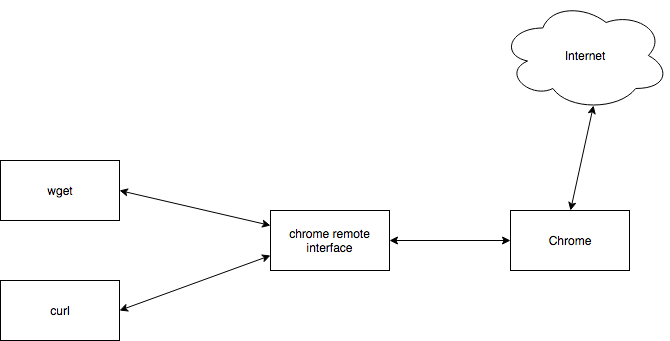
\includegraphics[width=\textwidth]{figures/prototype}
  \caption[Prototype approach]{\textbf{Prototype approach:} Applications issue
  requests and fetch responses from chrome through the chrome remote debugging
  protocol. Chrome makes the request on the application's behalf and fetches
  handles all connection security specifics.}
  \label{fig:prototype-saber}
\end{figure}

\subsection{Linking directly to chrome's networking code}
A more optimized approach would be to link directly with chrome's networking
library. This could potentially be more lightweight as it would only require
a small subset of chrome wrapped with a thin request API that applications
could interface with. \Cref{fig:long-term-saber} shows a potential design for
this approach. We omit this approach for future work.

\begin{figure}[h]
  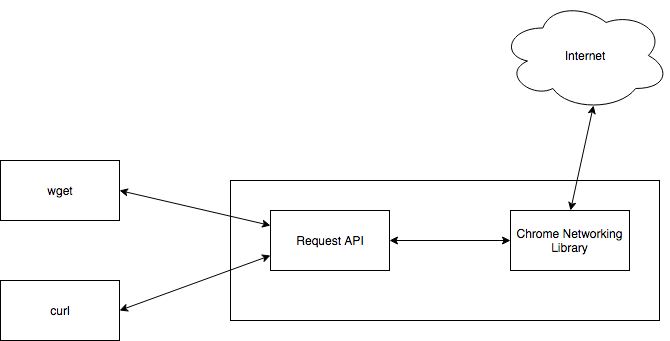
\includegraphics[width=\textwidth]{figures/long-term} \caption[Optimal
  approach]{\textbf{Optimal approach:} The network request library from chrome
  is exported (along with any security handling logic) and wrapped up in a
  library with an exposed Request API that non-browser applications interfact
  with.} \label{fig:long-term-saber}
\end{figure}

\subsection{Motivation}
The motivation behind our delegation is based on two key facts: (1) Browsers
are already pioneers of providing secure communication and other applications
can capitalize on that. (2) Writing security critical code is difficult and we
want to minimize the amount of such code that needs to be written by
developers. As an example, we implement \emph{swget}, a prototype of wget that
provides connection security without writing any TLS verification code.

\section{swget}
\label{sec:swget-saber}

\emph{wget} is a popular command line tool for downloading files from a
webserver. It is frequently used by developers to crawl web pages, download
scripts, and sometimes directly pipe such scripts to the shell. While such a
practice of executing code obtained remotely can be dangerous in itself, it
is especially a problem if the security of the connection is compromised by a
man-in-the middle attacker.

We wrote our own prototype version of \emph{secure wget} that has the same
basic functionality as wget, but uses chrome to make network requests. Looking
at wget's source code, we see it has 994 lines of code for interfacing with the
\emph{OpenSSL} library. Our version of swget uses the remote debugging protocol
to allow chrome to make requests on behalf of wget. We override chrome's
certificate handling settings using the remote debugging protocol to grab the
certificate error determined by chrome and cancel the request. We used the
chrome remote interface Node library to construct our messages to Chrome, which
allowed us to give \emph{swget} secure validation logic in only 8 lines of
application layer code.


\begin{figure}[h]
  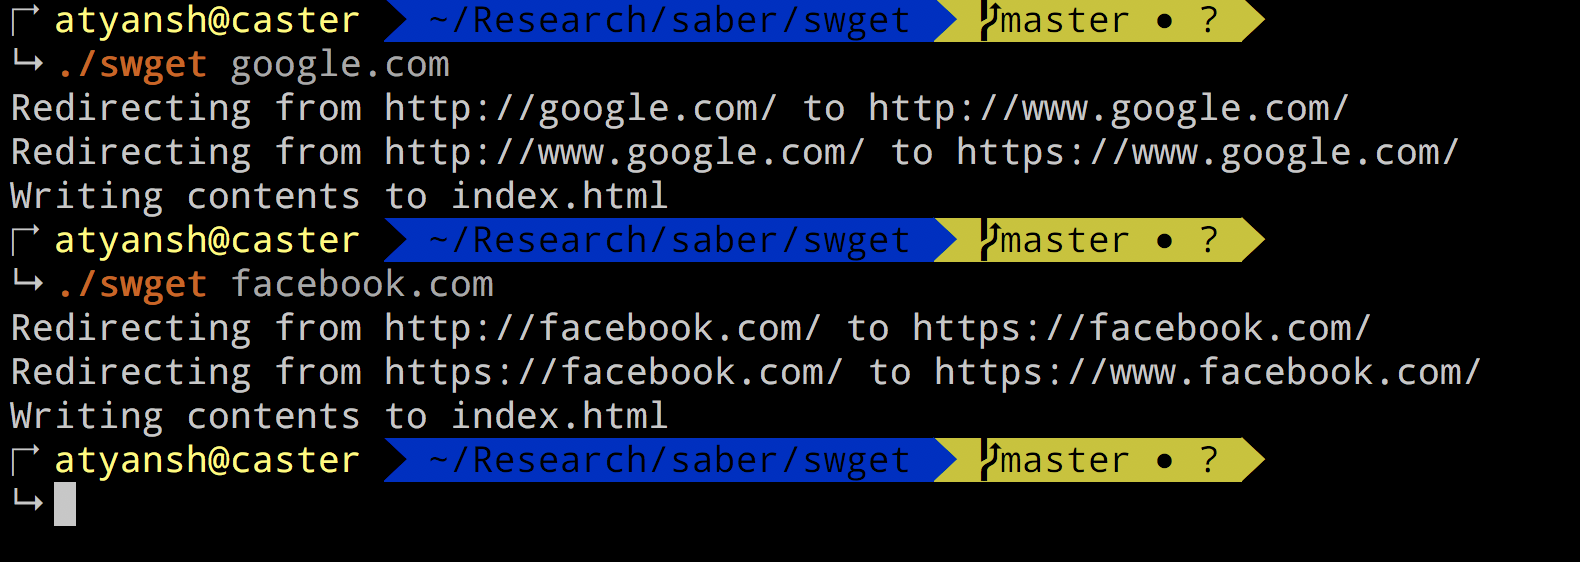
\includegraphics[width=\textwidth]{figures/regular}
  \caption[Regular usage of swget]{swget fetches and saves the webpage similar
  to wget in the normal case}
  \label{fig:regular-saber}
\end{figure}

Since chrome does certificate validation, swget's connection security is at
least as restrictive as chrome by default (although we can manually increase or
decrease restrictions based on what the application requires). This also
includes protection from revoked certificates, something which wget does not
provide today. A full list of our certificate testing for various applications
can be found in \Cref{app:results}.

\begin{figure}[h]
  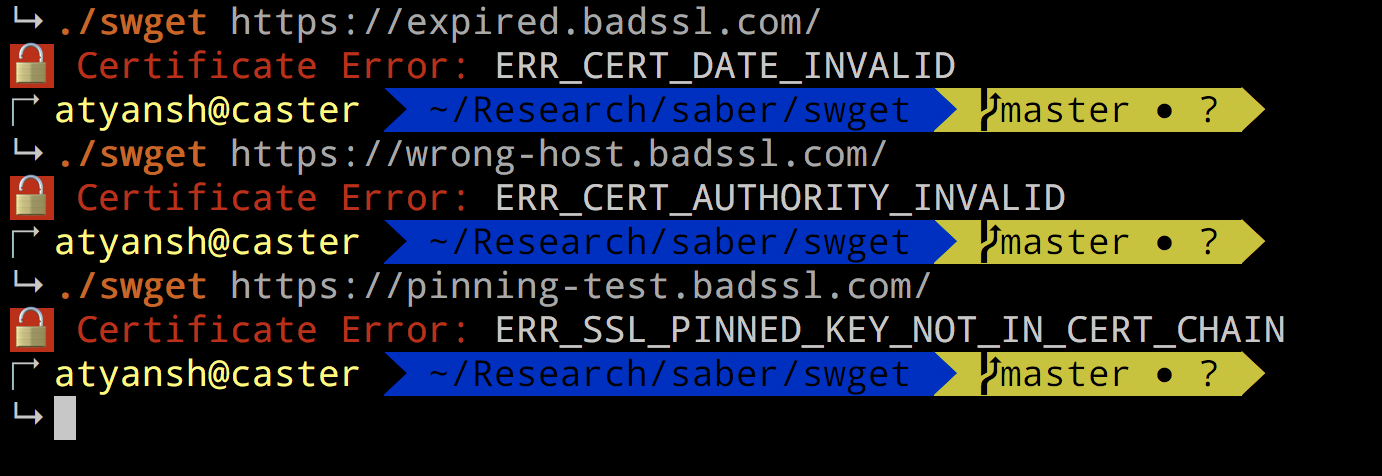
\includegraphics[width=\textwidth]{figures/cert-error}
  \caption[Behavior on certificate errors]{swget catches any certificate errors
  caught by chrome. In the figure, we see an example of domains with expired
  certificate, mismatched hostname, and an example of website that serves a
  valid certificate that was not pinned as part of the HPKP policy.} 
  \label{fig:cert-error-saber}
\end{figure}


\subsection{Secure redirects}
The default redirect behavior for chrome is for top level requests is to follow
redirects. While this behavior is okay for chrome, this may not be ideal for an
application like swget. Users use wget to fetch and download files. If a
request to fetch was made for an https link which was then redirected to http,
security of the connection could be compromised by an attacker. While browsers
can display the current security status to the user, there's no convenient way
to check whether a file downloaded with wget was actually downloaded securely
or not, once the file has already been fetched. We disable HTTPS to HTTP
redirects by default in our implementation of swget. As seen from
\Cref{fig:redirect-saber} a connection is terminated if the application
encounters an unsafe redirect.

\begin{figure}[h]
  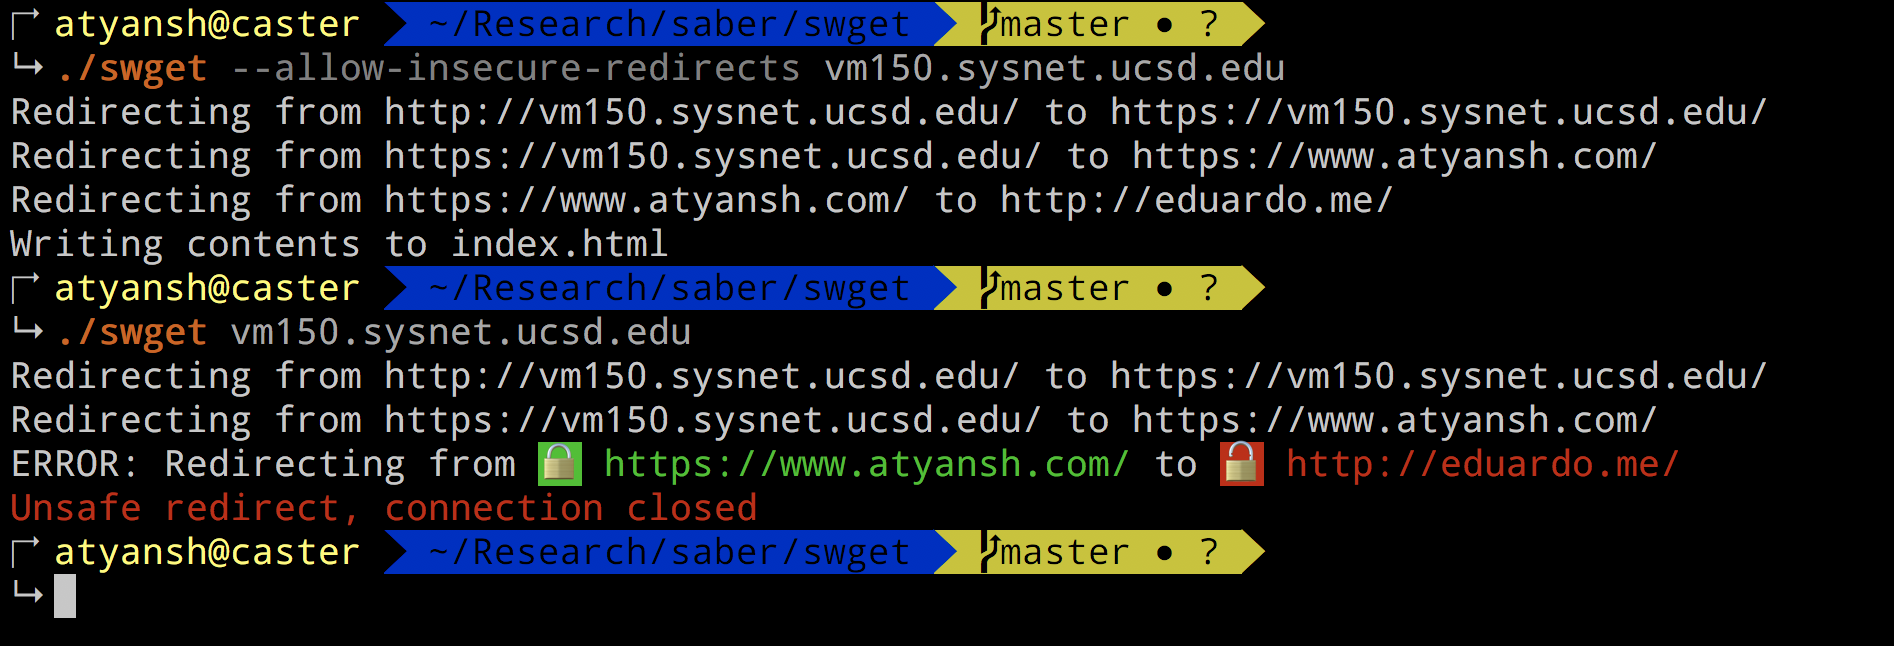
\includegraphics[width=\textwidth]{figures/redirect}
  \caption{Preventing unsafe https to http redirects} 
  \label{fig:redirect-saber}
\end{figure}

\subsection{Warning messages}
Non-browser applications have suffered from having poor UI in comparison to
browsers. Previous research has shown that better browser TLS warnings
decreased user click-through. We believe that improving warning messages for
users that use non-browser applications would benefit from improved warning
messages as well and have included more visual indicators (such as lock symbols)
to convey the security state of the connection. This is especially noticeable
in the case of redirects (\Cref{fig:redirect-saber}) and malware warnings
(\Cref{fig:malware-saber}). Further work needs to be done to measure the
effectiveness of these warnings.

\begin{figure}[h]
  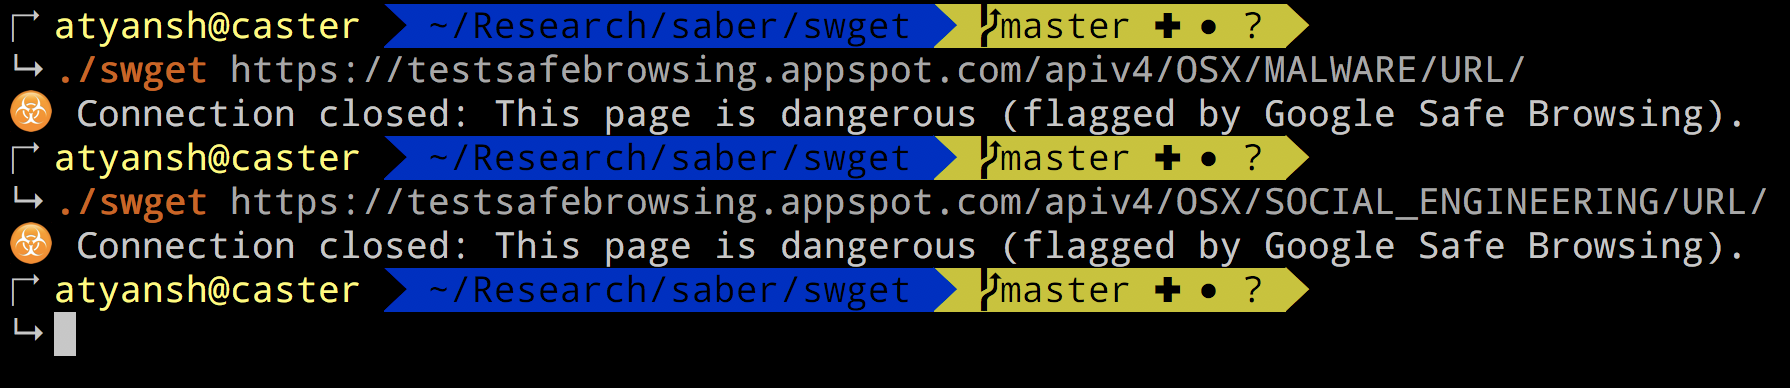
\includegraphics[width=\textwidth]{figures/malware}
  \caption{Malware detection as flagged by Chrome} 
  \label{fig:malware-saber}
\end{figure}

\subsection{Cookies and basic authentication}
Since swget uses chrome to issue 

\subsection{Global HSTS and HPKP}


\begin{figure}[h]
  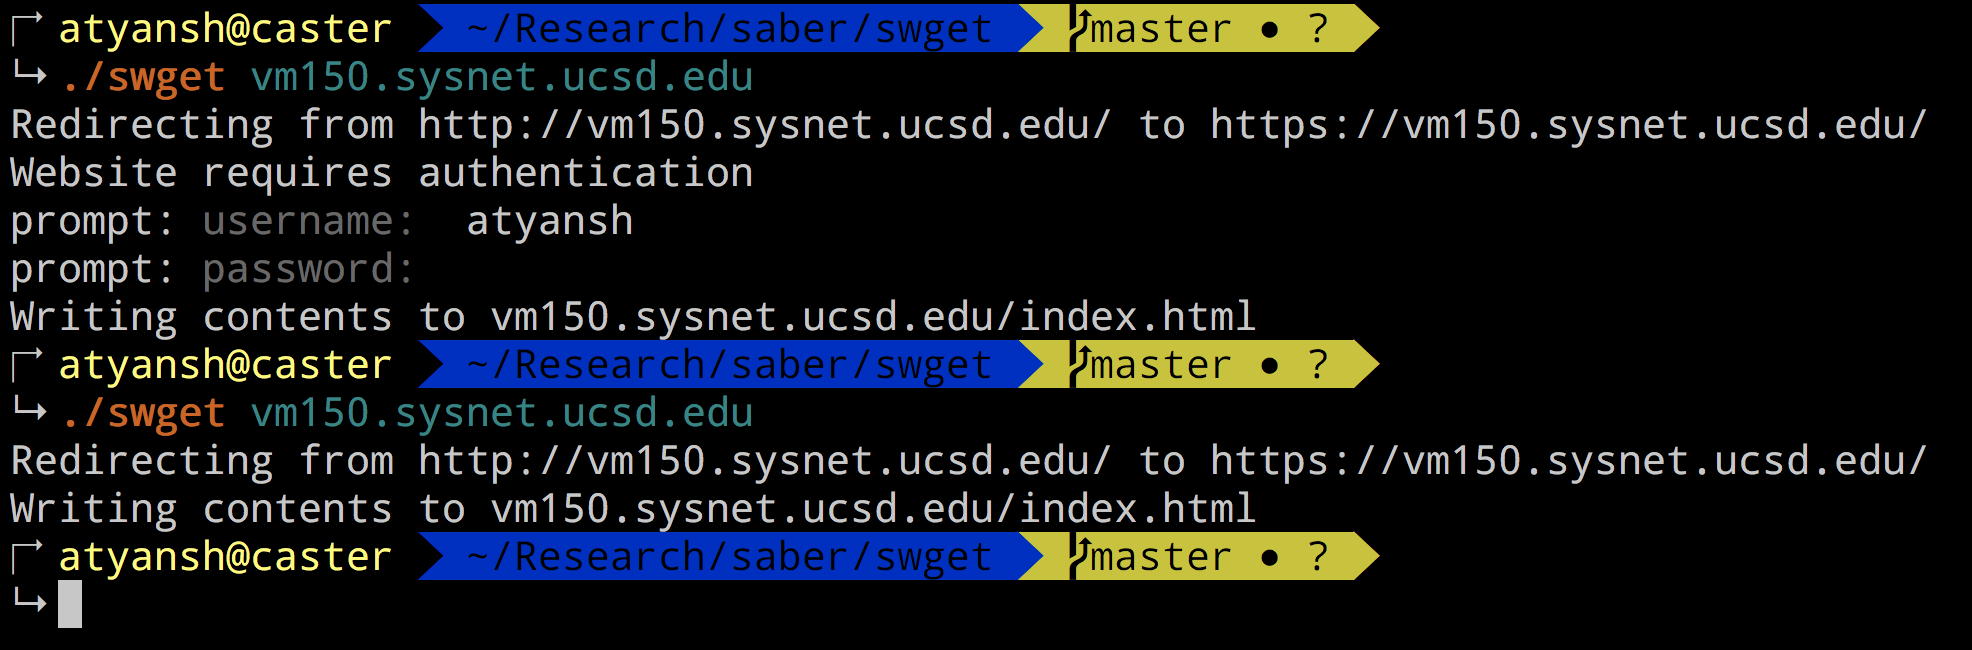
\includegraphics[width=\textwidth]{figures/basic-auth}
  \caption{HTTP Basic Auth} 
  \label{fig:basic-auth-saber}
\end{figure}


\section{Limitations}

\section{Conclusion}
\label{sec:conclusion-saber}

\section{Related Work}
\label{sec:related-saber}
